\documentclass{article}
\usepackage{graphicx}


\begin{document}
\begin{titlepage}
   \vspace*{\stretch{3.0}}
   \begin{center}
      \Large\textbf{CTARA Koregaon Project 2016}\\
      
      \large\textbf{Prof. Vikram M. Gadre}
      
      \large\textit{Koustubh Dwivedy, Sarthak Jain, Abhishek Khadiya}
      
      \large\textit{Swadesh Singh, Preshit Gulgulia, Angothu Prasanna}
   \end{center}
   \vspace*{\stretch{3.0}}
\end{titlepage}

\tableofcontents

\newpage
\section{Introduction}
Over the Academic Year 2015-16, two TDSL (Technology and Development Supervised Learning) teams have contributed to the development of the village of Koregaon near Satara, based on a nearby village named Kapshi. This TDSL effort intends to continue that endeavour.

\subsection{Location}
Koregaon village is located in the Satara district at distance of 45 km from Satara town and is 90km
south of Pune. Village lies in the leeward side of Mahadeo hills.
\begin{figure}[h]
\begin{center}
  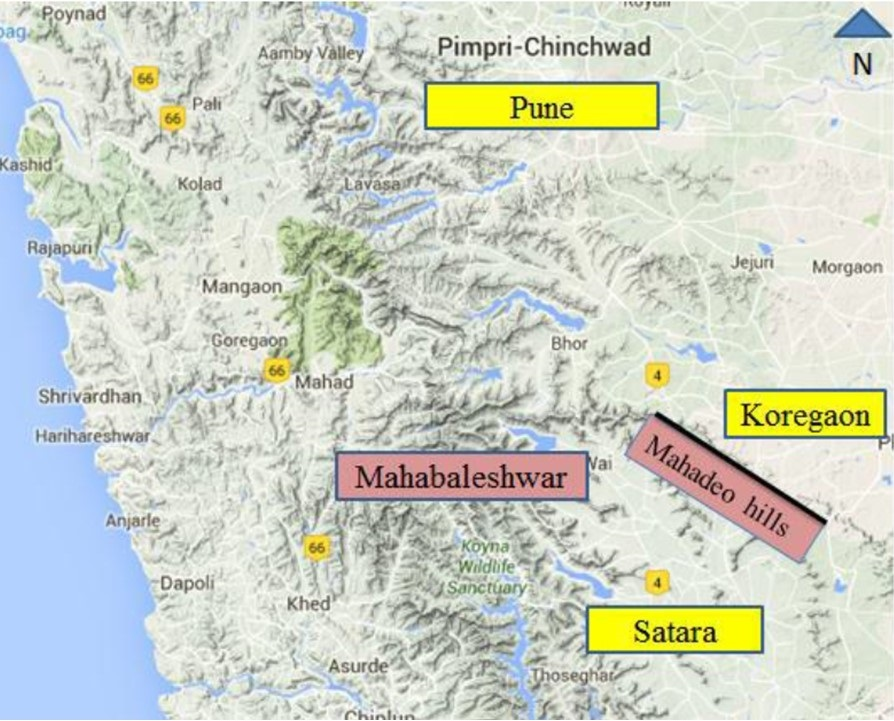
\includegraphics[scale=0.4]{images/location.jpg}
\end{center}
\end{figure}

\subsection{Project Description}
The aim of this project is to bring overall development of the Koregaon village. This village suffers from
water shortage which affects their agricultural production which is mostly onion. It was found that the
village does not have any onion storage facility. Past year's team worked on developing infrastructure to solve the problem of onion storage. Our team's aim is to deal with the problem of water shortage.
\section{Situation Review}
Koregaon village is one the most badly drought affected areas. The annual rainfall at the place is quite minimal and is hardly sufficient for the people to meet their demands. The situation is even worsened during the summers. While regions like Mahableshwar which are close to Sahayadri hills in west, receive rainfall as high as 2223 mm, moving eastwards the rainfall amount drops to less than 900 mm in the Taluka of Koregaon, Karad,Satara and to less than 600 mm in the Taluka of Man, Khatav, Phaltan and Khandala.
\subsection{Dependence on Monsoon Rains}
Currently Koregaon is dependent heavily on the monsoon rain. There are two small seasonal streams which run besides the village. There is small lake just outside the village which was constructed by government in 1960’s when the entire district was under severe drought. This small lake doesn’t have a good catchment area and with poor rainfall it gets dry within few months after monsoon season. Government had constructed two Bandharas (stop dams) on one of the stream but those failed within a year of operation. There are number of wells along the stream. These wells are dug to store the percolated water from stream. However due to rocky terrain the percolation is poor in these wells. So the villagers have put a bore well to meet the need of water. But this is leading to continuous decrease in the level of water table.

Looking at the much higher construction cost for the canal, the option to electrically pump the water from the stream to the lake seems to be significantly cheaper and feasible. In order to select the specifications of the pump we will visit the place and look at the geographical features of the area of interest. The lake existing in the village is very shallow and due to high temperature conditions in summer, the evaporation losses are significant since most of the surface areas is exposed to sun due to less depth.

The water collected in this lake would come from a nearby stream that remains dry for most of the year but fills up during the rainy season. The proposed solution is to transfer the water from the stream to the lake through pump.

\section{Methodology and Plan}

\section{Design and Implementation}

\end{document}